\documentclass[tikz,border=4pt]{standalone}
\usepackage{amsmath}
\begin{document}
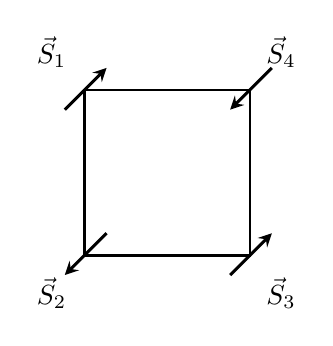
\begin{tikzpicture}[>=stealth, thick, scale=1.0]
  % Square connecting four spins: S1 top-left, S2 bottom-left, S3 bottom-right, S4 top-right
  \draw[line width=0.9pt] (0, 0) rectangle (2.1, 2.1);

  % Spin arrows at the four vertices
  \draw[->, line width=1.1pt] (-0.25, 1.85) -- (0.28, 2.38);
  \draw[->, line width=1.1pt] (0.28, 0.28) -- (-0.25, -0.25);
  \draw[->, line width=1.1pt] (1.85, -0.25) -- (2.38, 0.28);
  \draw[->, line width=1.1pt] (2.38, 2.38) -- (1.85, 1.85);

  \node[above left] at (-0.10, 2.25) {$\vec{S}_1$};
  \node[below left] at (-0.10, -0.15) {$\vec{S}_2$};
  \node[below right] at (2.18, -0.15) {$\vec{S}_3$};
  \node[above right] at (2.18, 2.25) {$\vec{S}_4$};
\end{tikzpicture}
\end{document}
